\documentclass[10pt,a4paper]{article}

% Packages
\usepackage[margin=1cm]{geometry} % Adjust margins as needed
\usepackage{url}
\usepackage{ragged2e} % For left-aligning text
\usepackage{authblk} % For multiple authors
\usepackage{hyperref}
\usepackage{longtable}
\usepackage{amsmath}
\usepackage{float}
\usepackage{graphicx}
\usepackage{caption}
\usepackage{subcaption}


\setlength{\parskip}{1em plus 0.2em minus 0.1em}
\setlength{\parindent}{0pt}

% Left-align all text
\RaggedRight

\begin{document}
% Title and author information
\title{CM22010 2024/2025 S1 Report}
\author{Christopher Gladman}
\author{Thomas Turner}
\author{Sultan Fawad}
\author{Maya Hargreaves}
\author{Grigorii Grachev}
\affil{University of Bath}
\maketitle

\section{Curves and Surfaces}

\subsection{Curve Representations}
We begin with parametric and implicit curve representations. Parametric representations consist of a set of variables which can each be modulated to fit the curve shape, and implicit curves are constituted by a finite set of points. Parametric curves are used extensively to represent smooth curves with a small memory footprint, for example, smooth glyphs composed of curved sections on large displays, such as the English letter ‘d’.  Implicit representations of geometry are used extensively in collision detection, such as the popular AABB algorithm. For a direct comparison, we utilised numpy’s built in \texttt{linspace} and \texttt{meshgrid} functions, generating 2000 evenly spaced points on the interval \texttt{[-10, 10]} on both the x and y axes for which an implicit and parametric circle could be evaluated. We then merged two circle shapes, which will include any intersections, by taking the product of the two implicit circles, and stitching the two parametric circles.


\begin{figure}[H]
\centering
\begin{subfigure}[b]{0.20\textwidth}
    \centering
    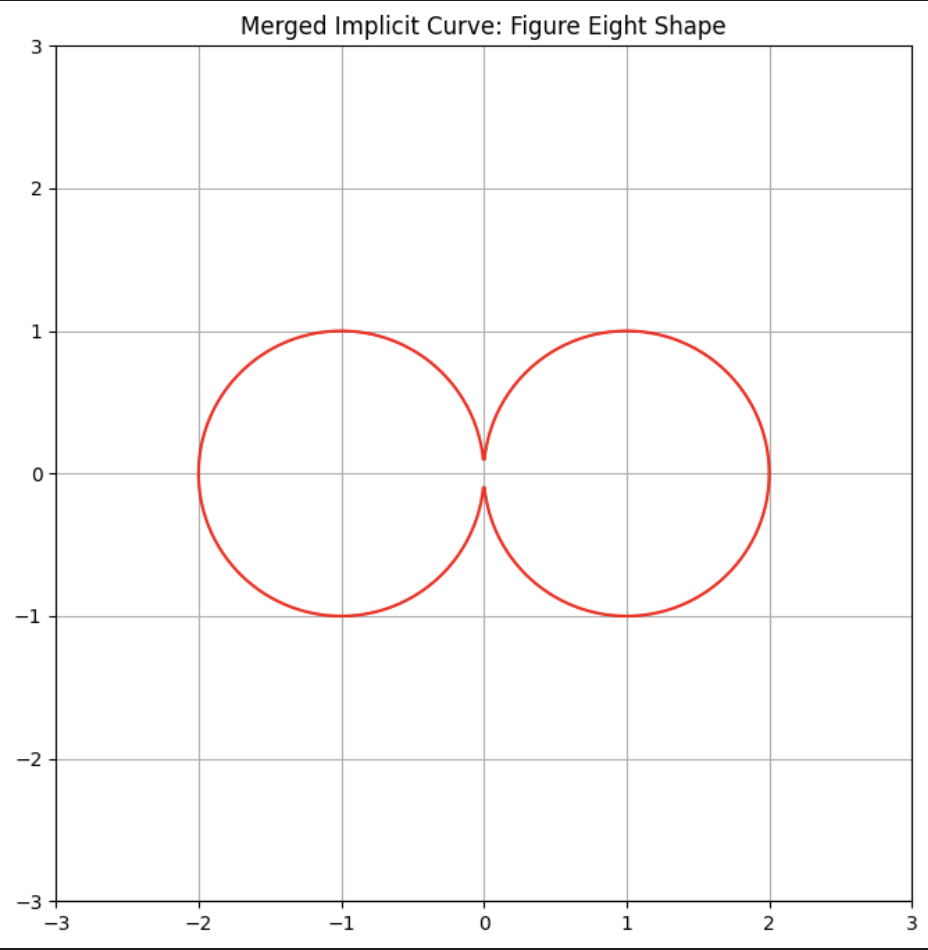
\includegraphics[width=\textwidth]{VisualComputingReportResults/ImplicitShapeMerging}
    \caption{\small Implicit Shape Merging}
    \label{fig:cubic}
\end{subfigure}
\hspace{0.1\textwidth}
\begin{subfigure}[b]{0.20\textwidth}
    \centering
    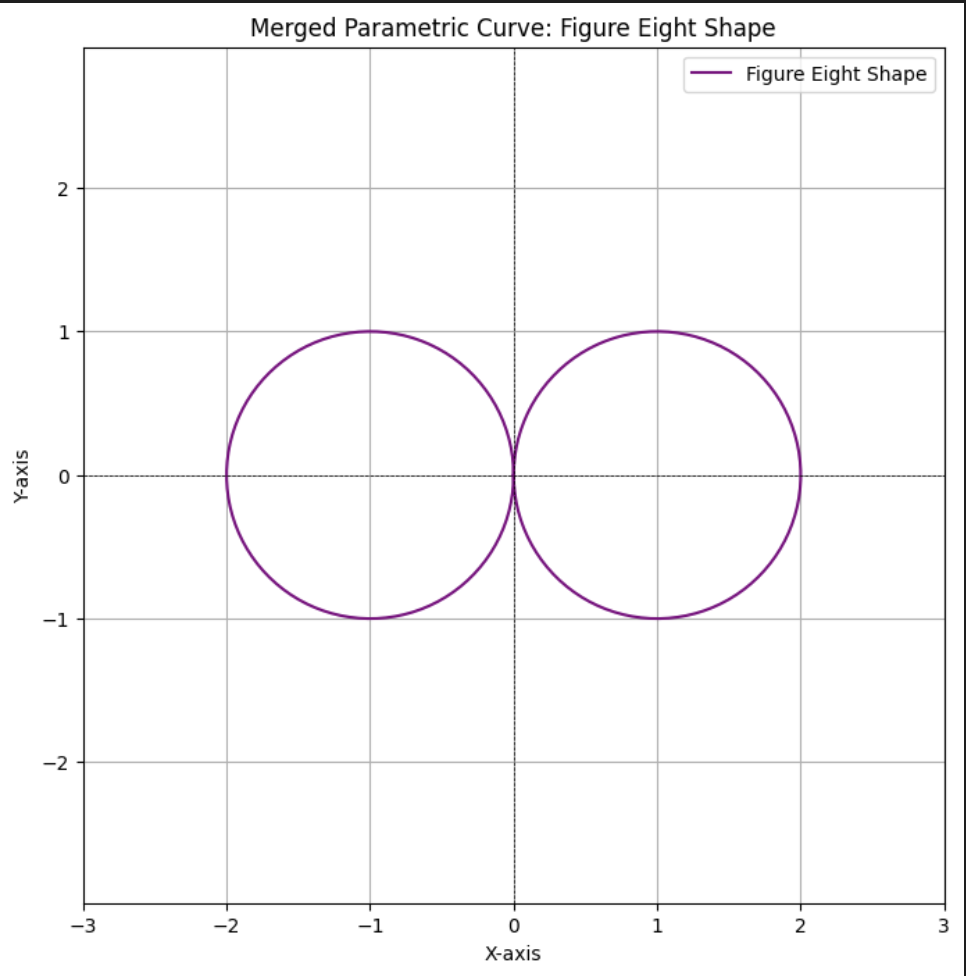
\includegraphics[width=\textwidth]{VisualComputingReportResults/ParametricShapeMerging}
    \caption{\small Parametric Shape Merging}
    \label{fig:quartic}
\end{subfigure}
\caption{\small Figure-Eight Shape Merge}
\label{fig:bezier_curves}
\end{figure}

Overall, it was demonstrated the parametric forms performed better for shape merging, maintaining a continuous figure-eight, whereas small precision errors in the implicit product led to some invalid values being produced at the intersections. It was also demonstrated through this that implicit representations would be more effective for intersection checking.

Also, as mentioned prior, parametric representations are beneficial in the context of generating smooth and cyclical curves. To demonstrate this, an attempt at generating a cycloid curve (commonly used for 2-dimensional wheel motion animations) was made for both a parametric and implicit representation. The cycloid path was simple to produce with the following parametric equations:

\begin{equation}
\begin{aligned}
x &= R(t - \sin t) \
y &= R(1 - \cos t)
\end{aligned}
\end{equation}

Producing the following cycloid shape over two complete cycles:

\begin{figure}[H]
\centering
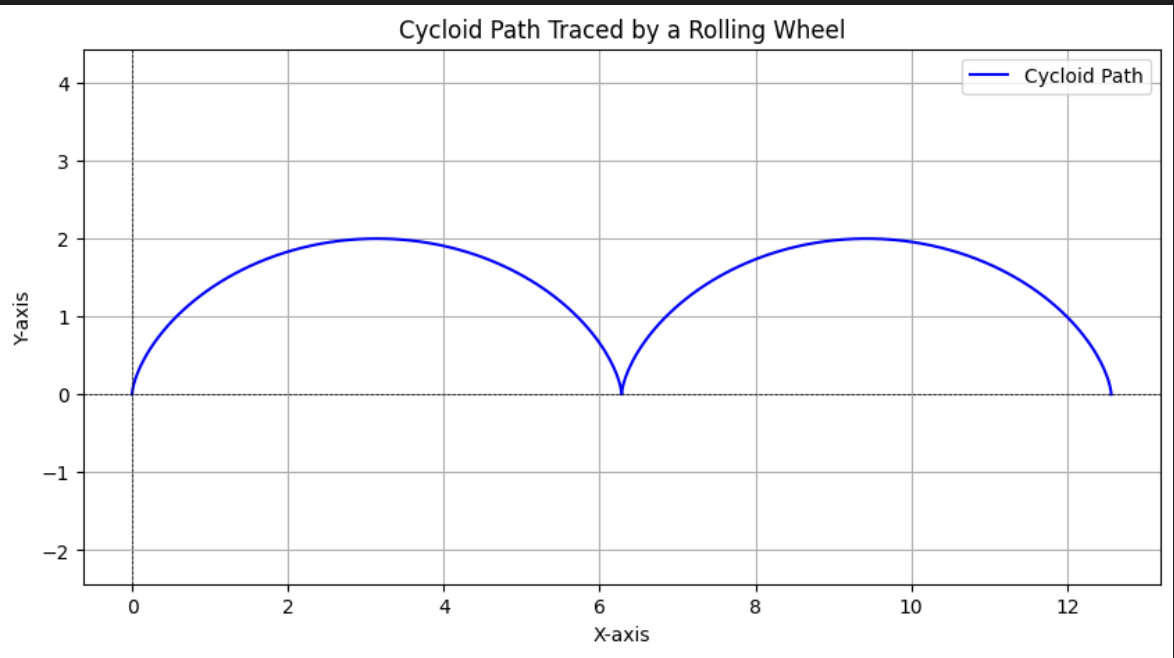
\includegraphics[width=0.48\textwidth]{VisualComputingReportResults/CycloidShape}
\caption{Cycloid curve generated over the interval [0, $4\pi$]}
\label{fig:your_label}
\end{figure}

The implicit representation, however, was impossible to produce accurately. It could not maintain periodicity, and required a repeated copying over of particular curve segments, leading to numerous discontinuities in the final curve.

\subsection{Cubic and Quartic Bezier Curves}

The notebook then progresses to particular parametric curve representations, Bezier curves and Hermite curves. Bezier curves are used extensively in smooth curve generation, with particular application in animation pathing. 

A set of control points were used to modulate the curve shape, which included the start of the curve, intermediary points and the endpoint of the curve. For each unique parameter in a parameter array generated by \texttt{numpy.linspace}, we compute the Bernstein basis polynomial:

\begin{equation}
b_{\nu,n}(x) = \binom{n}{\nu} x^{\nu} (1-x)^{n-\nu}, \quad \nu = 0, \ldots, n
\end{equation}

In practice, scipy's \texttt{comb} function was used to implement the combinatorial function. This polynomial value is computed for every control point with the parameter and is used to create a running sum which evaluates to the final \texttt{(x, y)} position on the curve. This in effect ‘pulls’ each parameter toward the control points.

Now, in order to define the cubic and quartic cases singularly, we complete the same process, except we define the Bernstein basis polynomials for degrees n=3 and n=4 explicitly. For example, the explicit formula for degree n=3 is given in Appendix A.

Finally, we must also ensure that we pass an appropriate number of control points to the Bezier curve algorithm, where the number of control points should be equivalent to one more than the degree of the polynomial. For results, below plotted are visual test cases for a cubic Bezier and quartic Bezier with control points provided as captions:

\begin{figure}[H]
\centering
\begin{subfigure}[b]{0.25\textwidth}
    \centering
    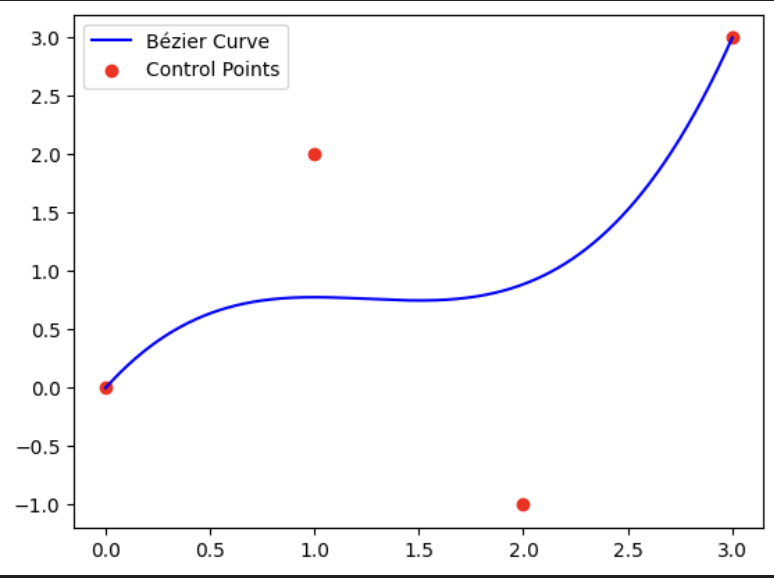
\includegraphics[width=\textwidth,height=0.25\textheight,keepaspectratio]{VisualComputingReportResults/CubicBezierCurve}
    \caption{\small [[0, 0], [1, 2], [2, -1], [3, 3]]}
    \label{fig:cubic}
\end{subfigure}
\hspace{0.1\textwidth}
\begin{subfigure}[b]{0.25\textwidth}
    \centering
    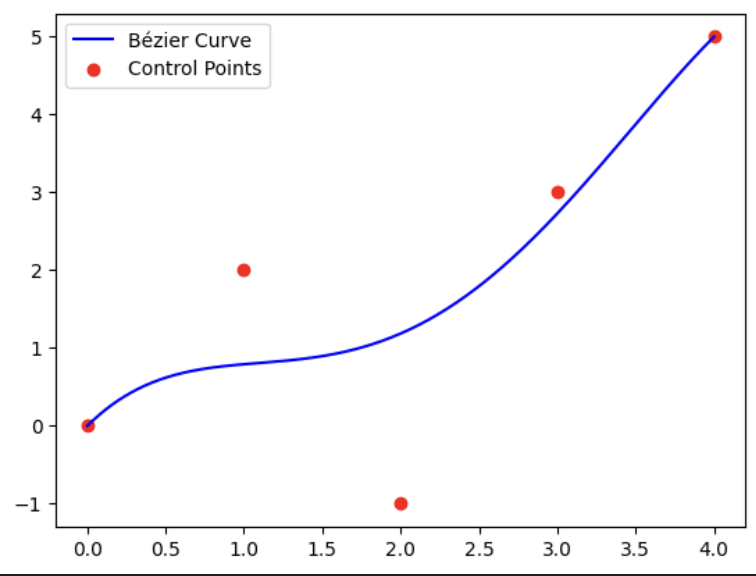
\includegraphics[width=\textwidth,height=0.25\textheight,keepaspectratio]{VisualComputingReportResults/QuarticBezierCurve}
    \caption{\small [[0, 0], [1, 2], [2, -1], [3, 3], [4, 5]]}
    \label{fig:quartic}
\end{subfigure}
\caption{\small Bezier Curves}
\label{fig:bezier_curves}
\end{figure}



\subsection{Hermite Curves}

Hermite curve representations are applied widely and are particularly useful where the user needs to specify the slope information directly by modifying the tangent vectors at each endpoint of the curve. For example, Hermite curves are preferred over Bezier curves in CAD (computer-aided design) applications, since curve segments can be modified independently, enabling finer local control of the curve.  

Similarly to the Bezier curve implementation, we first define a parametric array consisting of values \texttt{t}, in this case on the interval \texttt{[0, 1]} with some number of points defined (in our experimentation \texttt{n=100}). We then define the four Hermite basis functions, here for PCHIP (Piecewise Cubic Hermite Interpolating Polynomial), which is given in Appendix A. These are obtained by starting with the general definition of a cubic polynomial and applying necessary constraints, including the evaluation of endpoints at \texttt{t=0}, and the endpoint tangent vectors fitting the appropriate gradients such that $C_{1}$ continuity is maintained, and solving the resultant system of equations

A weighted sum of these basis functions with the endpoints and tangent vectors are then computed to calculate the point on the curve for each unique parameter. The formula is provided in Appendix A. Since Hermite curve shapes are determined by their endpoints and tangents (start, endpoint, start tangent, end tangent), their representations are highly flexible to tangent modifications. In order to experimentally test this, four Hermite curves were generated with the endpoints [0, 1] and varied tangent modifications.

\begin{figure}[H]
\centering
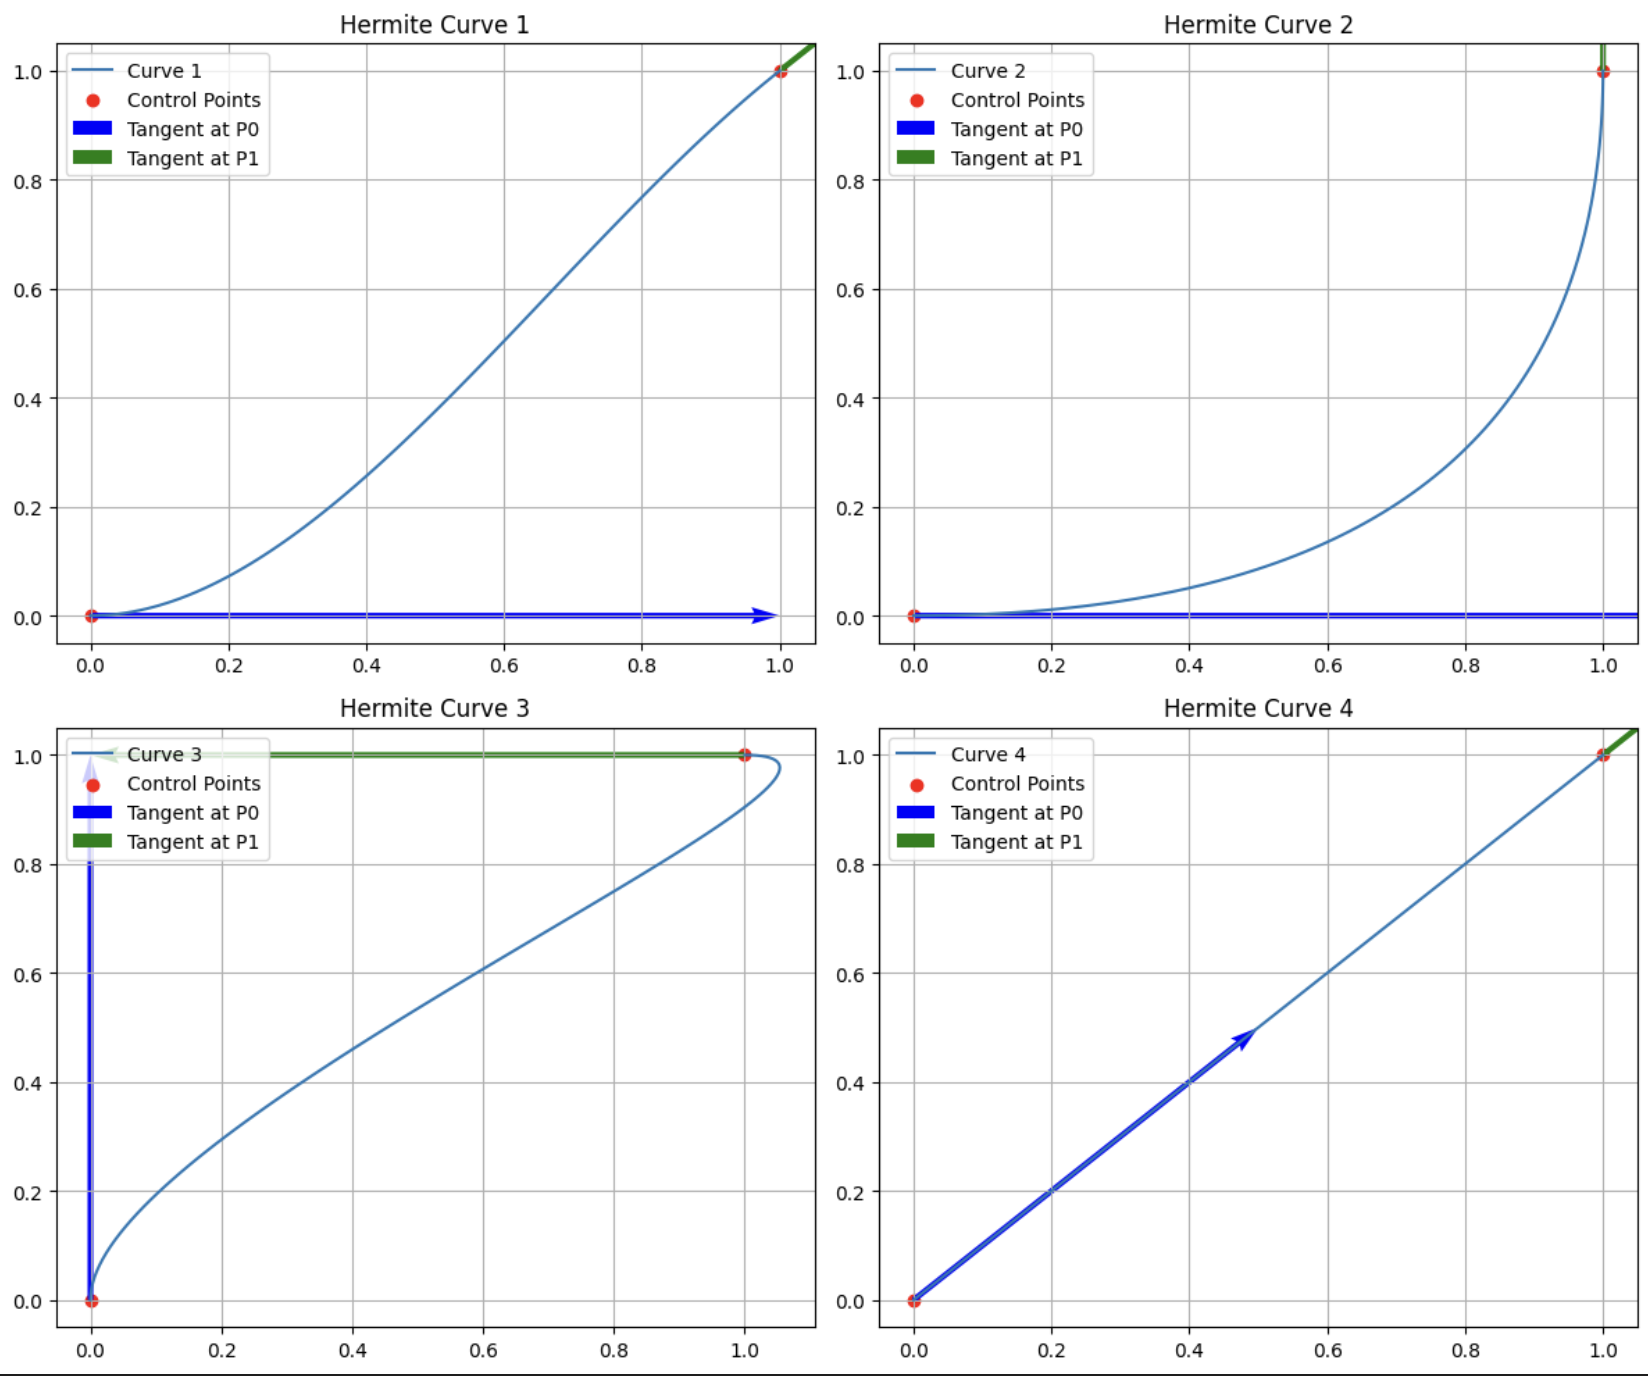
\includegraphics[width=0.5\textwidth]{VisualComputingReportResults/HermiteCurves}
\caption{Top Left: Original Test Case Tangents, Top Right: Exaggerated, Bottom Left: Vertical, Bottom Right: Parallel}
\label{fig:your_label}
\end{figure}

\subsection{Surface Extraction and Marching Cubes}

We then progress to surface extraction, which generally means to obtain surface geometry. This will be discussed in more formal detail in the theory section. Surface extraction is applied extensively in context of various medical imaging techniques. For example, CT (computed tomography) is able to support analysis of particular anatomical structures (i.e. differentiating bone from soft tissues) by obtaining 2D slices at different density values, a form of surface extraction known as iso-surfacing.  A particular algorithm known as Marching Cubes is then implemented which provides this functionality.  We were first tasked to implement a simple function which could extract surfaces from a scalar field. Firstly, we implemented a particular surface function, which decides the points which sit on, in or outside the surface. This effectively partitions the set of all points in a region of space into the interior ($<0$), boundary ($=0$), and exterior ($>0$). We decided to use the surface function for a torus, which is formally defined in Appendix A(iii). Then, for the simple case, we only needed to evaluate the zero-level set of the surface function, that is where it evaluates to zero. However, since some values will be arbitrarily close to zero but not exactly zero, it was required we defined a reasonable tolerance range (in this case any value $<0.0001$ is accepted as in the zero-level set). Finally, numpy’s built-in functions \texttt{isclose} and \texttt{where} enabled the selection of scalars in the surface function in this range.

\begin{figure}[H]
\centering
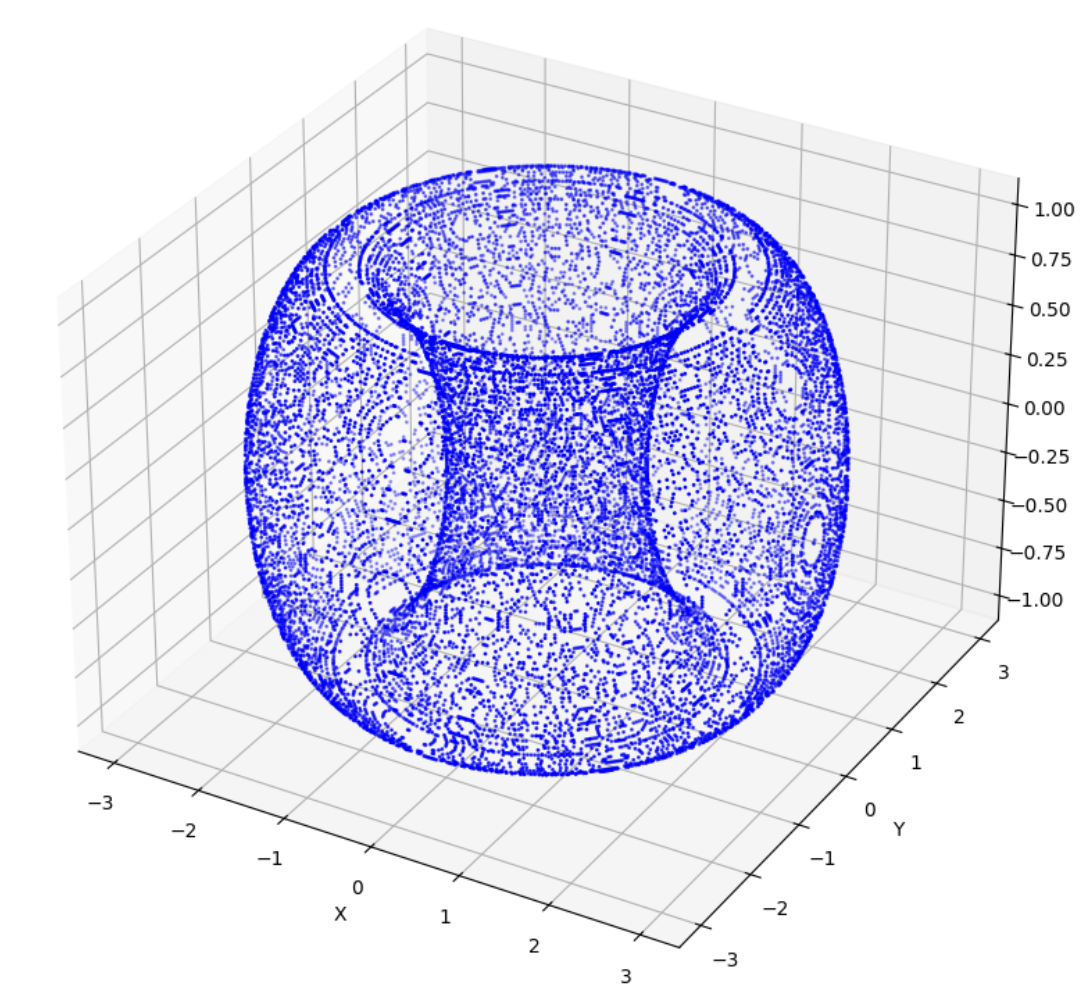
\includegraphics[width=0.20\textwidth]{VisualComputingReportResults/SimpleSurfaceExtraction}
\caption{Simple scalar field surface extraction at resolution \texttt{500x500x500}}
\label{fig:your_label}
\end{figure}

In the second part of this task, we were asked to implement the Marching Cubes Algorithm as a more efficiently computed and well-faithed representation of a surface. For each voxel, the coordinates of its centre and its corresponding vertices are extracted using this information as well as the spacing measurement between centre points, which is simple to compute from the resolution of the field. For example, the bottom-left-front vertex from the centre can be computed by subtracting the spacing from all three centre coordinates and halving them.

Next, whether the voxel is contained in the volume of interest or not is determined by comparing the iso-value with the density of the voxel. If the density is greater than the iso-value, it means that the voxel is outside of our volume of interest and we discount it in actual extraction. However, if our voxel is in our volume of interest, we now extract the surface by triangulating the voxel depending on a set of possible configurations. These configurations are whether each individual vertex of the voxel is inside or outside the iso-surface (full or empty respectively). In the three-dimensional case, there are 8 vertices,  generating $2^8= 256$ unique triangulations. Once these cases have been generated, they will serve as a lookup table using a binary mask.

In order to apply the triangulation, a trilinear interpolation is used. Interpolation is completed for each individual edge of each individual triangle produced as a result of the previous step. Firstly, the absolute differences between the densities of the vertices constituting the edge are checked, if it is arbitrarily close to zero (in our case $<0.0000001$), then we simply return the first point in the pair. Next, we compute \texttt{t}, a parameter that represents how far along the line segment between $p_{1}$ and $p_{2}$ we need to interpolate to reach the iso-value.

Marching Cubes was tested against multiple surface functions, with excellent results for the complex torus geometry, displayed below:


\begin{figure}[H]
\centering
\begin{subfigure}[b]{0.30\textwidth}
    \centering
    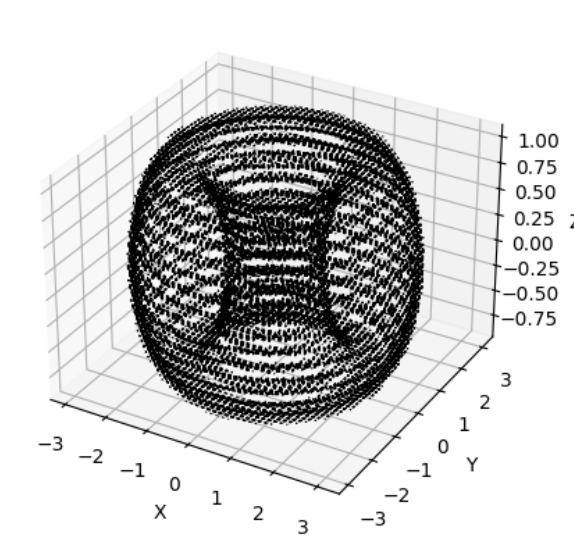
\includegraphics[width=\textwidth]{VisualComputingReportResults/MarchingCubesResolution50}
    \caption{\small Resolution=50}
    \label{fig:cubic}
\end{subfigure}
\hspace{0.1\textwidth}
\begin{subfigure}[b]{0.30\textwidth}
    \centering
    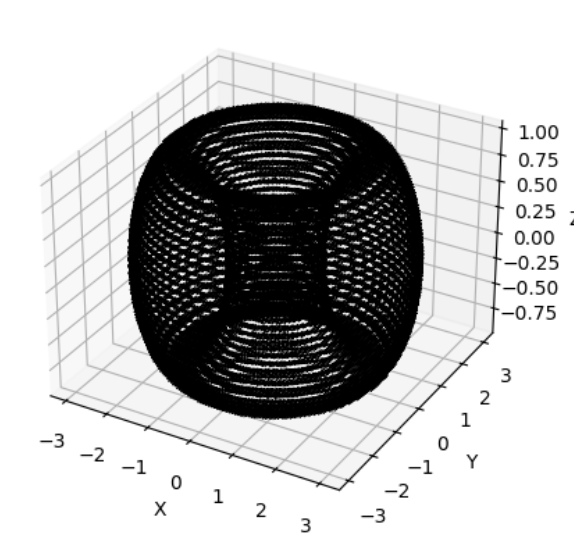
\includegraphics[width=\textwidth]{VisualComputingReportResults/MarchingCubesResolution100}
    \caption{\small Resolution=100}
    \label{fig:quartic}
\end{subfigure}
\caption{\small Marching Cubes}
\label{fig:bezier_curves}
\end{figure}


One note for a further improvement is that not all triangulation cases need to be stored explicitly, as the 256 configurations can be reduced to 15 unique cases as a result of rotational symmetries. 


\subsection{Subdivision Surfaces and Catmull-Clark} 

The final section considers a technique known as ‘subdivision surfaces’. This efers to the complexification of mesh geometry through the repeated subdivision of surface information into a collection of smaller but still topologically valid shapes, most commonly triangles or quadrilaterals. These techniques are used extensively, for example with Pixar animated characters and simulations of astrophysical objects, since a simpler ‘control’ mesh can be repeatedly refined to a more detailed target mash.

Our first task was to use a pre-built library to implement subdivision. For this, we utilised the \texttt{trimesh} library, which provided functionality for loading pre-defined control meshes, as well as an in-built implementation of the Catmull-Clark subdivision algorithm. Firstly, a low-polygonal control mesh of a rabbit is loaded from a ‘.obj’ file, following this, the \texttt{remesh.subdivide\_loop} method provides the functionality for continual subdivision. Multiple rounds of subdivision and the subsequent results for the mesh are displayed below, and these demonstrated the improvement of the visual quality and smoothness of the rabbit model, to a level of granularity that would not be perceptible for the casual viewer of an animated film which may utilise such a model as a background object:

(IMAGE TO GO HERE)

We were then tasked to implement Catmull-Clark without external library support. The Catmull Clark algorithm first begins by computing a set of face points, which are in essence the mean average over the set of vertices that contribute to a face. Next, the algorithm will produce edge points. It first generates all possible edges using the face information, assuming that the vertices in each face are stored in counter-clockwise winding order, which is the case in the initialisation of the example unit cube provided. It does this by simply pairing each adjacent set of vertices.

Now, provided we have generated the edges correctly, we will have two distinct cases to handle for edge points, where the edge is bordering a hole, and where it is not. A hole is simply referring to a gap in the mesh surface. Edge detection for holes is simple through determining the number of faces the edge belongs to. If this is only one face, then the edge is bordering a hole, otherwise it is not. In the case where the edge is bordering a hole, we generate the edge point as the mean of the vertices constituting that edge. Otherwise, we generate the edge point by computing the mean of the face points of each face containing the edge, alongside the edge centre.

Next, we compute the locations of the new vertices of the subdivided mesh. This again is partitioned into the case of vertices bordering versus not bordering a hole. Finally, each face of the original mesh is replaced by a quadrilateral face, but both cases must be dealt with separately.  Three new quadrilateral faces replace the original triangular face, and four new quadrilateral faces replace the original quadrilateral face. The formulae for these is provided in Appendix ...

The effectiveness of the algorithm was tested using three repeated applications of subdivision on the unit cube, as this was simple to compare against other visual examples of a correct Catmull-Clark implementation. This yielded, as to be expected, a continuous refinement of the original cube into an even spherical shape:

\begin{figure}[H]
\centering
\begin{subfigure}[b]{0.25\textwidth}
    \centering
    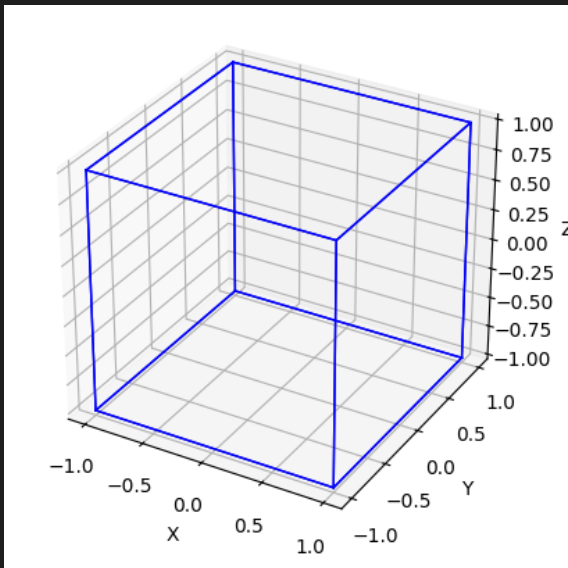
\includegraphics[width=\textwidth]{VisualComputingReportResults/CatmullClarkInitialUnitCube}
    \caption{\small Unit Cube}
    \label{fig:cubic}
\end{subfigure}
\hspace{0.2\textwidth}
\begin{subfigure}[b]{0.25\textwidth}
    \centering
    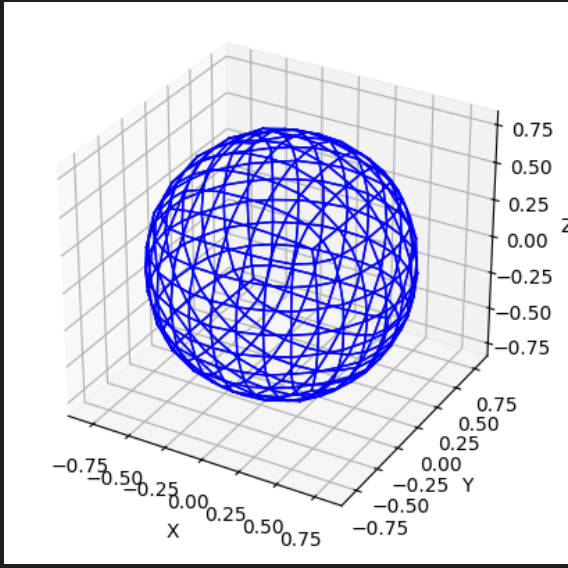
\includegraphics[width=\textwidth]{VisualComputingReportResults/CatmullClarkThirdSubdivision}
    \caption{\small Third Subdivision}
    \label{fig:quartic}
\end{subfigure}
\caption{\small Catmull-Clark Subdivision}
\label{fig:bezier_curves}
\end{figure}



\section{Transforms}

Matrices are an intuitive and powerful tool used to mathematically represent transformations. In effect, they allow us to alter shapes constituent vectors relative to the vector spaces standard basis, thereby allowing us to scale, shear, translate, rotate and apply non-affine transformations to objects. They constitute one of the most fundamental principles in computer graphics, facilitating the representation of movement on both absolute and relative scales. 
This section details transformations in the vector space R(to the power)2, representing 2-dimensional Euclidean space. Such mechanisms form the basis of 2-D vector graphics, seeing wide application in everything from animation to logo design. 


\subsection{Basic Translation Matrices}

\begin{table}[h]
\centering
\begin{tabular}{|c|c|c|}
\hline
Name & Homogeneous form & Representation \\
\hline
Translation & 
$T = \begin{bmatrix}
1 & 0 & a \\
0 & 1 & b \\
0 & 0 & 1
\end{bmatrix}$ & 
$\begin{bmatrix}
x' \\
y'
\end{bmatrix} = 
\begin{bmatrix}
x \\
y
\end{bmatrix} + 
\begin{bmatrix}
a \\
b
\end{bmatrix}$ \\
\hline
Rotation (Counterclockwise / Radians) & 
$R = \begin{bmatrix}
\cos\phi & -\sin\phi & 0 \\
\sin\phi & \cos\phi & 0 \\
0 & 0 & 1
\end{bmatrix}$ & 
$\begin{bmatrix}
x' \\
y'
\end{bmatrix} = 
\begin{bmatrix}
x \\
y
\end{bmatrix} \cdot 
\begin{bmatrix}
\cos\phi & -\sin\phi \\
\sin\phi & \cos\phi
\end{bmatrix}$ \\
\hline
Scaling (uniform) & 
$s = \begin{bmatrix}
n & 0 & 0 \\
0 & n & 0 \\
0 & 0 & 1
\end{bmatrix}$ & 
$\begin{bmatrix}
x' \\
y'
\end{bmatrix} = 
\begin{bmatrix}
x \\
y
\end{bmatrix} \cdot 
\begin{bmatrix}
n & 0 \\
0 & n
\end{bmatrix}$ \\
\hline
\end{tabular}
\caption{Transformation Matrices and Their Representations}
\label{tab:transformations}
\end{table}

Task 1 implements these transformations through the scaling(scale...factor), translation(point) and rotation(angle)subroutines. Notably, the interface for rotation accepts angular measurements in degrees. All subroutines implement these transformations using homogenous matrix form, facilitating the creation of compound transformations in successive tasks. 

The functionality of these subroutines is validated through test cases in the Jupyter notebook.


\subsection{Composite Transformations}

Task 2 implements compound transformations in both pre- and post- multiplicative form through the \texttt{rotation\_scaling\_and\_translation} and the \\ \texttt{rotation\_scaling\_and\_translation\_postmultiplied} subroutines. Both routines are compositions of the functions defined in task 1, and follow standard transformation procedure, rotating before scaling and translating in column (pre) multiplication and inverting this order for row-wise (post) multiplication, as well as transposing the constituent matrices. Our compound transformation matrices are as follows:

\begin{align}
T_{\text{compound}} &= T \cdot S \cdot R \\
T_{\text{compound\_post}} &= R^T \cdot S^T \cdot T^T
\end{align}

Both implementations of compound transformation matrices yielded consistent results when given appropriately formatted input vectors, thus showcasing the versatility of matrices, across differing forms of representation. 

It was observed that applying transformations in the wrong order produced incorrect results. For example, applying translation before rotation caused shapes to rotate around an unintended pivot. This happens because matrix transformations do not possess the commutative property. 



\subsection{Articulated Motion}

Task 3’s subroutines aimed to simulate a system of objects in relative motion, particularly controlling the motion of the second and third moon orbiting the planet in the provided model. 

The second moon orbits the planet at 3 units distance and rotates twice as fast as the first moon. This is described by the \texttt{transform\_moon2($\theta$)} function the compound transformation is thus comprised of both a translation and a rotation.  \texttt{T\_earth}, given in this notebook, represents a rotation. The combined transformation is thus $T_{\text{moon2}} = T_{\text{earth}}(2\theta)$.
	 
The third moon orbits the second at 1 unit distance, rotating twice per animation cycle. This transformation implemented by the \texttt{transform\_moon3($\theta$)} subroutine, and is relative to the second moon, thus comprising the second moon’s transformation matrix, multiplied with an additional rotation and translation matrix, adjusted to achieve the previously stated results. The complete matrix is thus $T_{\text{moon3}} = T_{\text{moon2}}(\theta) \cdot R(\theta) \cdot T([1, 0])$.
	 
This simulation of a system demonstrates the power and utility of hierarchal transformations, with each object’s movement constituting of independent movements in conjunction to matrix describing the movement of its parent. It was noted that when using non-affine transformations, child objects displayed unexpected orbital paths. This is as non-affine transformations are non-uniform and do not maintain parallel lines, thus distorting movement. 


\subsection{Estimating Transforms}

This notebook focussed on creating combinations of previously defined functions to estimate the transformation between a start shape and a set of targets. As well as invoking these functions, additional transformation matrices were defined, describing non-uniform (axes-wise) scaling, shearing as well as non-affine transformations (through homographies). 

\begin{table}[H]
\centering
\begin{tabular}{|c|c|c|}
\hline
\textbf{Name} & \textbf{Subroutine} & \textbf{Representation} \\
\hline
X-wise scale & scaleX(sf) & $X_s = \begin{bmatrix} sf & 0 & 0 \\ 0 & 1 & 0 \\ 0 & 0 & 1 \end{bmatrix}$ \\
Y-wise scale & scaleY(sf) & $Y_s = \begin{bmatrix} 1 & 0 & 0 \\ 0 & sf & 0 \\ 0 & 0 & 1 \end{bmatrix}$ \\
Shear (A=x, B=y) & shearAB(a, b) & $SH = \begin{bmatrix} 1 & a & 0 \\ b & 1 & 0 \\ 0 & 0 & 1 \end{bmatrix}$ \\
Homography & Homography (non-affine, changes perspective) & $H = \begin{bmatrix} h_{11} & h_{12} & h_{13} \\ h_{21} & h_{22} & h_{23} \\ h_{31} & h_{32} & 1 \end{bmatrix}$ \\
\hline
\end{tabular}
\caption{Transformations for input vector in $R^2$}
\end{table}

\begin{table}[H]
\centering
\begin{tabular}{|c|c|}
\hline
\textbf{Shape} & \textbf{Transformation (Estimate)} \\
\hline
A & $T(5,1)$ \\
\hline
B & $T(7,0) \cdot S\left(\frac{1}{2.45}\right)$ \\
\hline
C & $T(9.5,1.55) \cdot X_s(1.2) \cdot Y_s(0.4)$ \\
\hline
D & $T(0,7) \cdot R(315^\circ)$ \\
\hline
E & $T(2,10) \cdot R(45^\circ) \cdot S(0.5)$ \\
\hline
F & $T(4,14) \cdot R(-135^\circ) \cdot X_s(0.4) \cdot Y_s(0.8)$ \\
\hline
G & $T(8,8) \cdot R(22.5^\circ) \cdot SH(0.01, 1.05) \cdot Y_s(0.685) \cdot X_s(0.95)$ \\
\hline
H & Homography $\sim \begin{bmatrix} 0.27 & 0 & -0.85 \\ -0.25 & -0.2 & 5.65 \\ -0.02 & -0.09 & 1 \end{bmatrix}$ \\
\hline
\end{tabular}
\caption{Shape Transformations (Estimates) using Matrices Defined in Tables}
\end{table}

Our estimates were largely concordant with the true transformations from the start shape to the corresponding letters. The transformations describing G and H, while within reasonable bounds, are not exact matches. 

It was observed that applying non-affine components to a composite affine transformation distorted the vector space, not maintaining the affine matrix components when combined by multiplication. To mitigate this issue, a standalone matrix was created for shape “H”, allowing individual elements to be edited independently, to achieve desired effects. 

We also considered some potential avenues for further experimentation. Including allowing user-defined parameters like angles, scale factors, and translations to modify animations interactively, extending the polygon library to include circles, ellipses, or irregular shapes, building more intricate articulated systems (e.g., solar systems with multiple planets, and transition from 2D to 3D transformations for enhanced applications like 3D modelling or robotics.

\section{Appendices}

\subsection{Appendix A}

\begin{align}
b_{0,3}(x) &= (1-x)^3 \\
b_{1,3}(x) &= 3x(1-x)^2 \\
b_{2,3}(x) &= 3x^2(1-x) \\
b_{3,3}(x) &= x^3
\end{align}

\begin{align}
H_{00}(t) &= (1 + 2t)(1 - t)^2 \\
H_{10}(t) &= t(1 - t)^2 \\
H_{01}(t) &= t^2(3 - 2t) \\
H_{11}(t) &= t^2(t - 1)
\end{align}

\begin{equation}
f(x, y, z) = \left(\sqrt{x^2 + y^2} - R\right)^2 + z^2 - r^2 
\end{equation}

Where \texttt{R} is the major radius (distance from center of tube to center of torus), \texttt{r} is the minor radius, \texttt{(x, y, z)} are the Cartesian coordinates.




\end{document}
